\begin{figure*}[t]
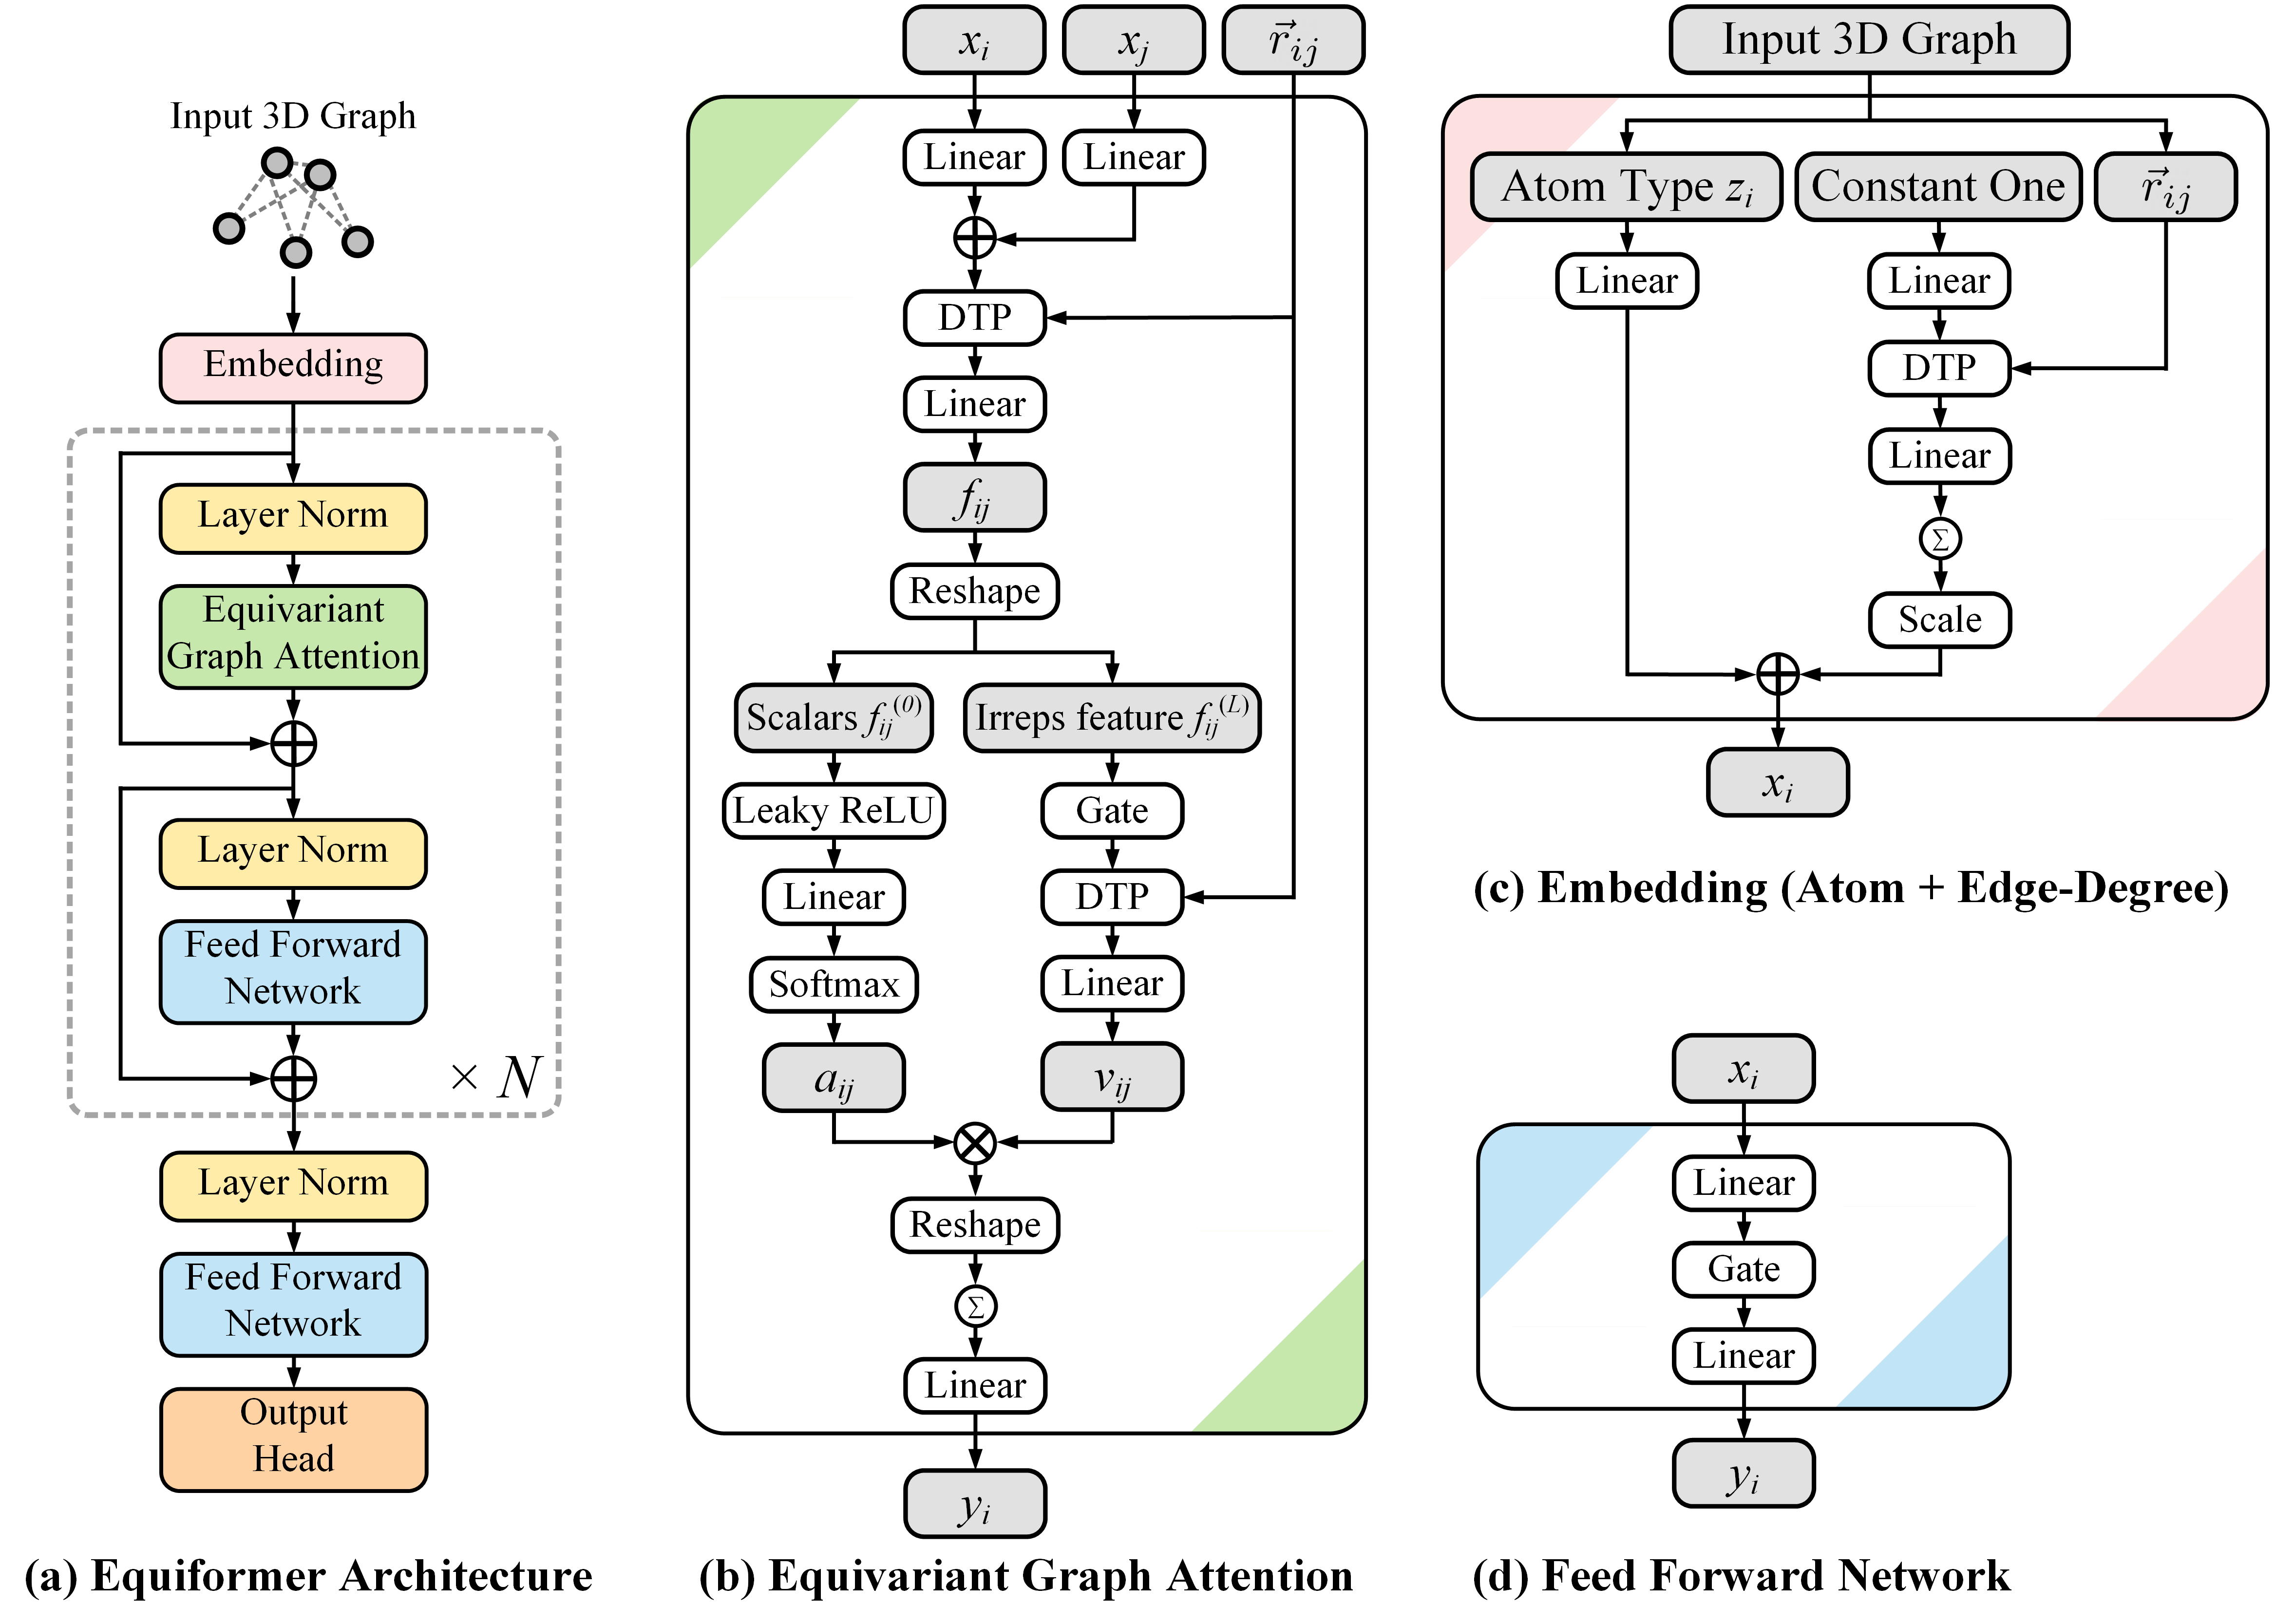
\includegraphics[width=0.75\linewidth]{figure/equiformer.png}
\centering
\vspace{-2.5mm}
\caption{\textbf{Architecture of Equiformer.}
We embed input 3D graphs with atom and edge-degree embeddings and process them with Transformer blocks, consisting of equivariant graph attention and feed forward networks.
In this figure, ``$\otimes$'' denotes multiplication, ``$\oplus$'' denotes addition, and ``DTP'' stands for depth-wise tensor product. $\sum$ within a circle denotes summation over all neighbors.
Gray cells indicate intermediate irreps features.
}
\vspace{-6mm}
\label{fig:equiformer}
\end{figure*}


\vspace{-4mm}
\section{Equiformer}
\vspace{-3mm}

\definecolor{mygreen}{RGB}{64, 179, 79}



%Starting from Transformer architecture~\cite{transformer}, we propose three modifications to obtain Equiformer as illustrated in Fig.~\ref{fig:equiformer}.
%First, we incorporate E(3) representations and change all original operations to their equivariant counterparts.
%Second, we propose a novel equivariant graph attention, which is more expressive than the original attention used in Transformer.
%Third, we propose edge-degree embedding to encode degree information, which can be hard to capture with pure attention.
%%%We incorporate $SE(3)$/$E(3)$-equivariant irreps features into Transformers~\citep{transformer} and use equivariant operations.
%To better adapt Transformer to 3D graph structures, we propose equivariant graph attention and edge-degree embedding.
%To better adapt Transformers to 3D graph structures, we propose equivariant graph attention.
\revision{First, we propose a simple and effective architecture, Equiformer with dot product attention and linear message passing, by only replacing original operations in Transformers with their equivariant counterparts and including tensor products for $SE(3)$/$E(3)$-equivariant irreps features.}
\revision{The equivariant operations are discussed in Sec.~\ref{subsec:equivariant_operations}.}
\revision{The equivariant version of dot product attention can be found in Sec.~\ref{appendix:subsec:dot_product_attention}, and that of other modules in Transformers can be found in Sec.~\ref{subsec:overall_architecture}.}
\revision{Second,} we propose a novel attention mechanism called equivariant graph attention \revision{in Sec.~\ref{subsec:equivariant_graph_attention}}.
\revision{The proposed Equiformer combines these two innovations and} is illustrated in Fig.~\ref{fig:equiformer}. 
%The overall architecture of Equiformer is illustrated in Fig.~\ref{fig:equiformer}. 

%\subsection{Incorporating E(3) Features}
\label{subsec:incorporate_e3_features}

\begin{figure*}[t]
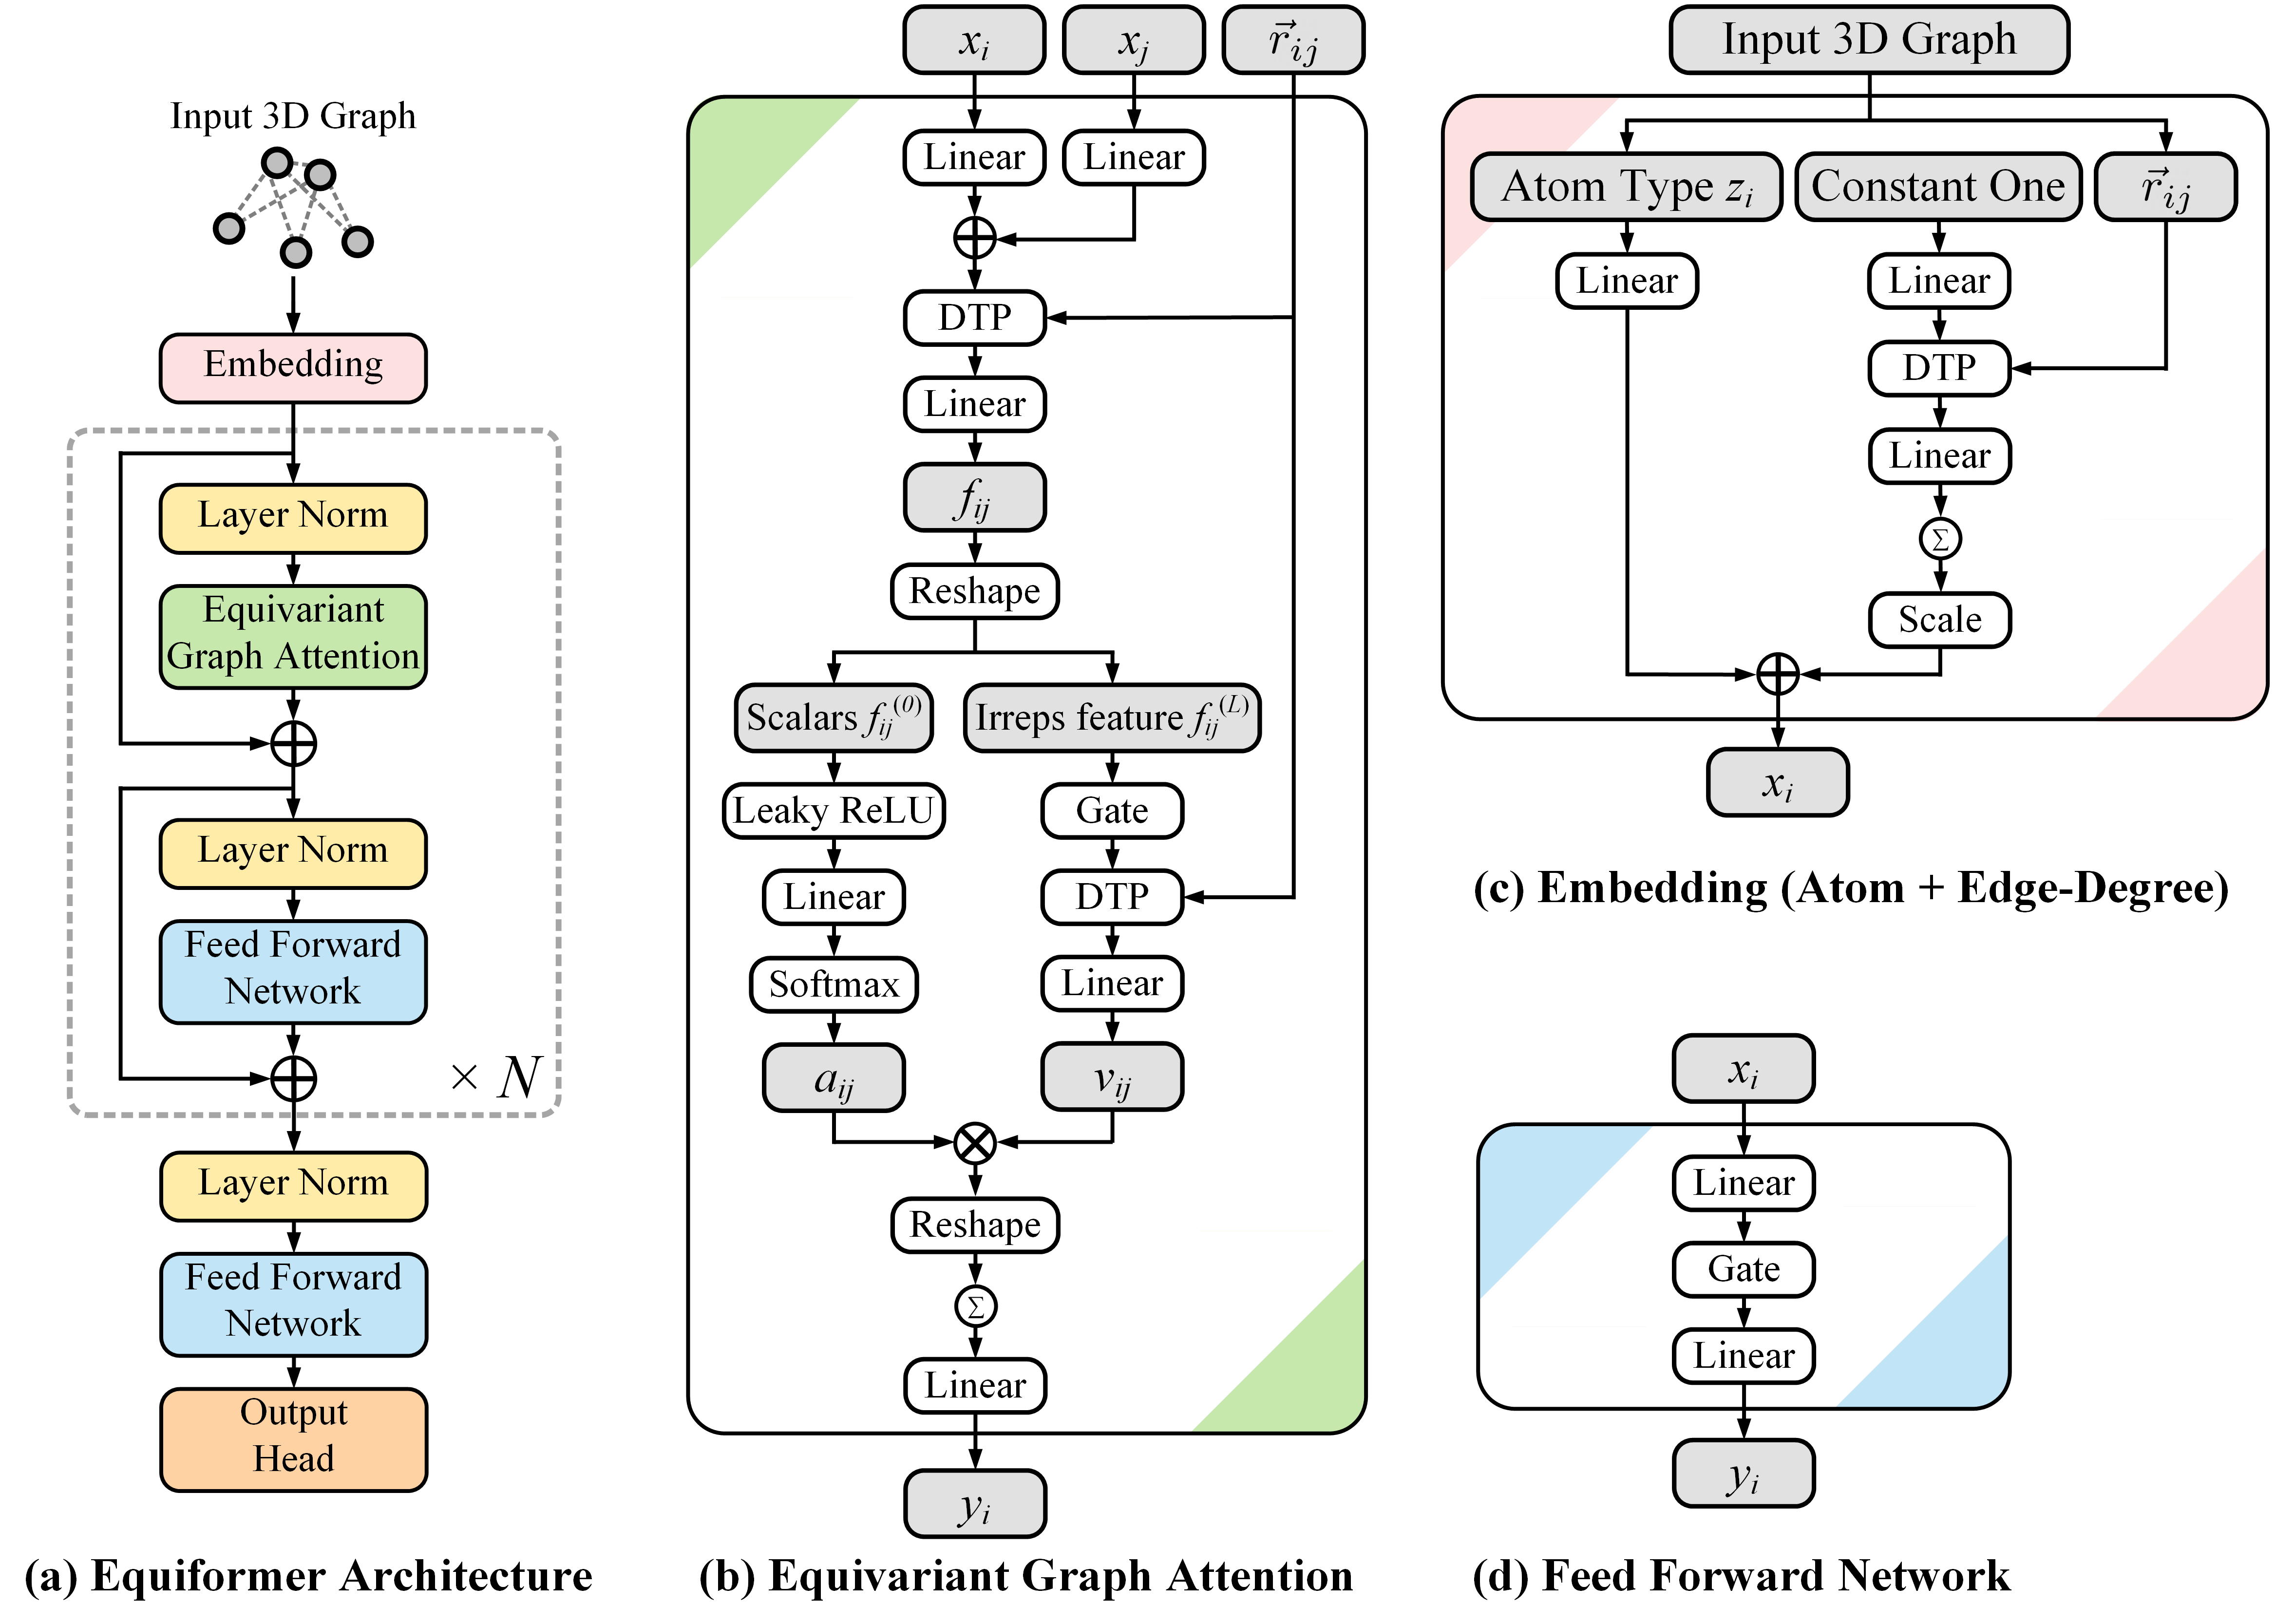
\includegraphics[width=0.9\linewidth]{figure/equiformer.png}
\centering
\caption{\textbf{Architecture of Equiformer.}
\todo{Add detailed explanation of each submodule of Attention to figures in Appendix.}
\todo{Add dot product attention in Appendix.}
\todo{Update variables: $x_{ij}, a_{ij}, v_{ij}$}
Here ``$\otimes$'' denotes multiplication, ``$\oplus$'' denotes addition, and ``DTP'' stands for depth-wise tensor product. $\sum$ within a circle denotes summation over all neighbors.
}
\label{fig:equiformer}
\end{figure*}

\begin{enumerate}
    \item \note{Typical GNN and Transformer operate on scalars}
    \item \note{Equivariance}
    \item \note{Including E(3)}
    \item \note{Picture for Linear, Gate, DTP, Layer Norm}
\end{enumerate}

\todo{May be moved to Background}

\todo{Definition of Graph and 3D Graph}


\paragraph{Directional Information.}
Typical graph neural networks (GNNs) use scalars as internal representations.
As scalars are invariant features, after geometric transformations like rotations, they will remain the same.
This means that the representations are insensitive to rotations and therefore cannot encode any directional information.
However, directional information contained in quantities like forces is indispensable to understand interactions between atoms from the perspective of physics.
Moreover, discarding directional information can make GNNs less expressive as they cannot differentiate certain types of graphs.
These motivate using other representations instead of only scalars.


\paragraph{Equivariance.}

\paragraph{E(3) Features.}

\vspace{-2.5mm}
\subsection{Equivariant Operations for Irreps Features}
\vspace{-2.5mm}
\label{subsec:equivariant_operations}

%As irreps features encode directional and equivariant information in channel dimensions without complicating graph structures, we can adopt irreps features and inherit the design of existing networks through utilizing equivariant operations.
\revision{We discuss below equivariant operations, which serve as building blocks for equivariant graph attention and other modules, and analyze how they remain equivariant in Sec.~\ref{appendix:subsec:equivariant_operations}.}
%They include the equivariant version of the original operations in Transformers and the depth-wise tensor product, as illustrated in Fig.~\ref{fig:equivariant_operation} in appendix. %, an efficient version of tensor product.
They include the equivariant version of operations in Transformers and depth-wise tensor products as shown in Fig.~\ref{fig:equivariant_operation}. % in appendix. %, an efficient version of tensor product.

%\note{(We describe the difference of the operations in Equiformer from what has already introduced in Background.)}

%Since the internal representations are E(3) features, we replace the original operations with equivariant counterparts to preserve E(3)-equivariance and discuss equivariant versions of operations used in Transformer.
%Besides, we adopt the operation of tensor product to exchange the information contained in different type-$l$ vectors.

%\todo{Add figure for each of them!}

\vspace{-2.5mm}
\paragraph{Linear.}
Linear layers are generalized to irreps features by transforming different type-$L$ vectors separately.
Specifically, we apply separate linear operations to each group of type-$L$ vectors.
We remove bias terms for non-scalar features with $L > 0$ as biases do not depend on inputs, and therefore, including biases for type-$L$ vectors with $L > 0$ can break equivariance.
%Note that linear layers can be regarded as a special case of tensor product between E(3) features and type-$0$ constant one.

\vspace{-2.5mm}
\paragraph{Layer Normalization.}
Transformers adopt layer normalization (LN)~\citep{layer_norm} to stabilize training.
%\revision{
%Given input $x \in \mathbb{R}^{N \times C}$, with $N$ being the number of nodes and $C$ the number of channels, LN  calculates the linear transformation of normalized input as follows:
Given input $x \in \mathbb{R}^{N \times C}$, with $N$ being the number of nodes and $C$ the number of channels, LN  calculates the linear transformation of normalized input as $\text{LN}(x) = \left( \frac{  x - \mu_{C}  }{\sigma_{C}} \right) \circ \gamma + \beta$,
%\begin{equation}
%\text{LN}(x) = \frac{x - \mu_{C}}{\sigma_{C}} \circ \gamma + \beta
%\end{equation}
where $\mu_{C}, \sigma_{C} \in \mathbb{R}^{N \times 1}$ are mean and standard deviation of input $x$ along the channel dimension, $\gamma, \beta \in \mathbb{R}^{1 \times C}$ are learnable parameters, and $\circ$ denotes element-wise product.
%}
By viewing standard deviation as the root mean square value (RMS) of L2-norm of type-$L$ vectors, LN can be generalized to irreps features.
Specifically, given input $x \in \mathbb{R}^{N \times C \times (2L + 1)}$ of type-$L$ vectors, the output is
$\text{LN}(x) = \left( \frac{x}{\text{RMS}_{C}(\text{norm}(x))} \right) \circ \gamma$,
%\begin{equation}
%\text{LN}(x) = \frac{x}{\text{RMS}_{C}(\text{norm}(x))} \circ \gamma
%\end{equation}
where $\text{norm}(x) \in \mathbb{R}^{N \times C \times 1}$ calculates the L2-norm of each type-$L$ vectors in $x$, and $\text{RMS}_{C}(\text{norm}(x)) \in \mathbb{R}^{N \times 1 \times 1}$ calculates the RMS of L2-norm with mean taken along the channel dimension.
%%%We remove mean and biases for type-$L$ vectors with $L \neq 0$ following linear layers.
We remove means and biases for type-$L$ vectors with $L \neq 0$.

\vspace{-2.5mm}
\paragraph{Gate.}
We use the gate activation~\citep{3dsteerable} for equivariant activation function as shown in Fig.~\ref{fig:equivariant_operation}(c).
Typical activation functions are applied to type-$0$ vectors.
For vectors of higher $L$, we multiply them with non-linearly transformed type-$0$ vectors for equivariance.
Specifically, given input $x$ containing non-scalar $C_{L}$ type-$L$ vectors with $ 0 < L \leq L_{max}$ and $(C_0 + \sum_{L=1}^{L_{max}} C_L)$ type-$0$ vectors, we apply SiLU~\citep{silu, swish} to the first $C_0$ type-$0$ vectors and sigmoid function to the other $\sum_{L=1}^{L_{max}} C_L$ type-$0$ vectors to obtain non-linear weights and multiply each type-$L$ vector with corresponding non-linear weights.
After the gate activation, the number of channels for type-$0$ vectors is reduced to $C_0$.

\vspace{-2.5mm}
\paragraph{Depth-wise Tensor Product.}
The tensor product defines interaction between vectors of different $L$.
%%%To improve its efficiency, we use the depth-wise tensor product (DTP), which restricts one type-$L$ vector in output irreps features depends only on one type-$L'$ vector in input irreps features, where $L$ can be equal to or different from $L'$.
To improve its efficiency, we use the depth-wise tensor product (DTP), where one type-$L$ vector in output irreps features depends only on one type-$L'$ vector in input irreps features as illustrated in Fig.~\ref{fig:equivariant_operation}(d) and Fig.~\ref{fig:depthwise_tensor_product_e3nn}, with $L$ being equal to or different from $L'$.
This is similar to depth-wise convolution~\citep{mobilenet}, where one output channel depends on only one input channel. 
%, and therefore, we call it depth-wise tensor product (DTP).
Weights $w$ in the DTP can be input-independent or conditioned on relative distances, and the DTP between two tensors $x$ and $y$ is denoted as $x \otimes_{w}^{DTP} y$. % $x \tens_{w}^{DTP} y$.
%\todo{(Mention tensor product weights in Background)}
Note that the one-to-one dependence of channels can significantly reduce the number of weights and thus memory complexity when weights are conditioned on relative distances.
In contrast, if one output channel depends on all input channels, in our case, this can lead to out-of-memory errors when weights are parametrized by relative distances.

\begin{figure*}[t]
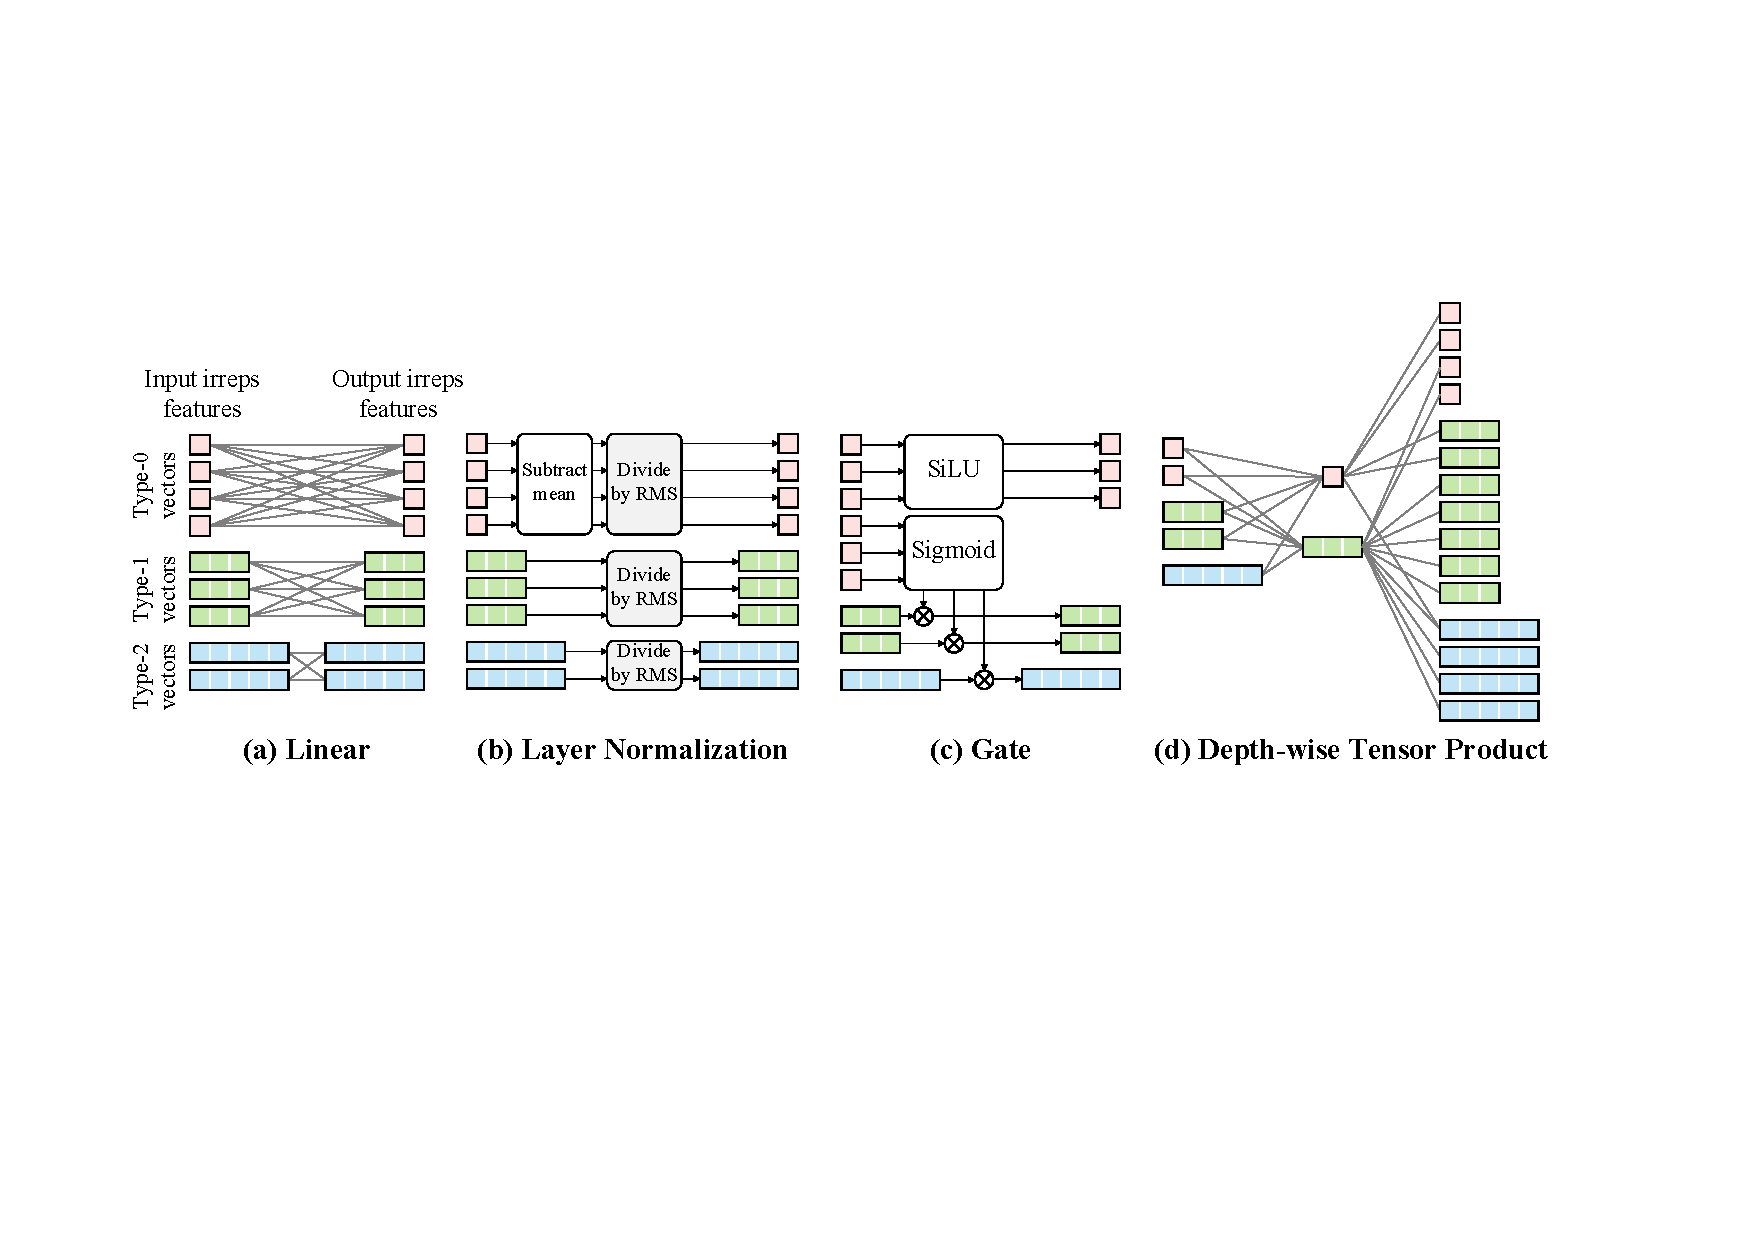
\includegraphics[width=0.85\linewidth]{figure/equivariant_operation.pdf}
\centering
\vspace{-3.5mm}
\caption{
\textbf{Equivariant operations used in Equiformer.}
%For ``Linear'', each gray line has one learnable weight.
\textbf{(a)} Each gray line between input and output irreps features contains one learnable weight.
%Note that the number of output channels can be different from that of input channels.
%The number of output channels can be different from that of input channels.
%For ``Layer Normalization'', ``RMS'' denotes root mean squared value with mean taken along channel dimension, and we remove multiplying by $\gamma$ in this figure for simplicity.  
%\textbf{(b)} ``RMS'' denotes the root mean square value (RMS) along the channel dimension.
\textbf{(b)} ``RMS'' denotes the root mean square value along the channel dimension.
For simplicity, we have removed multiplying by $\gamma$ here.
\textbf{(c)} Gate layers are equivariant activation functions where non-linearly transformed scalars are used to gate non-scalar irreps features.
\textbf{(d)} The left two irreps features correspond to two input irreps features, and the rightmost one is the output irreps feature.
%For ``Depth-wise Tensor Product'', the left two irreps features correspond to two input irreps features, and the rightmost one is output irreps feature.
The two gray lines connecting two vectors in the input irreps features and one vector in the output irreps feature form a path and contain one learnable weight.
An alternative visualization of depth-wise tensor products can be found in Fig.~\ref{fig:depthwise_tensor_product_e3nn} in appendix.
We show $SE(3)$-equivariant operations here, which can be generalized to $E(3)$-equivariant features.
}

\vspace{-4mm}
\label{fig:equivariant_operation}
\end{figure*}

\vspace{-3mm}
\subsection{Equivariant Graph Attention}
\label{subsec:equivariant_graph_attention}
\vspace{-2mm}

Self-attention~\citep{transformer, gat, se3_transformer, transformer_in_vision, graphormer, gatv2} transforms features sent from one spatial location to another with input-dependent weights.
We use the notion from Transformers~\citep{transformer} and message passing networks~\citep{neural_message_passing_quantum_chemistry} and define message $m_{ij}$ sent from node $j$ to node $i$ as follows:
\begin{equation}
m_{ij} = a_{ij} \times v_{ij}
\end{equation}
%where attention weights $a_{ij}$ depend on features on node $i$ and its neighbors $\mathcal{N}(i)$ and values $v_{ij}$ are features sent from node $j$ to node $i$ transformed with input-independent weights.
where attention weights $a_{ij}$ depend on features on node $i$ and its neighbors $\mathcal{N}(i)$ and values $v_{ij}$ are transformed with input-independent weights.
In Transformers and Graph Attention Networks (GAT)~\citep{gat, gatv2}, $v_{ij}$ depends only on node $j$.
In message passing networks~\citep{neural_message_passing_quantum_chemistry}, $v_{ij}$ depends on features on nodes $i$ and $j$ with constant $a_{ij}$.
The proposed equivariant graph attention adopts tensor products to incorporate content and geometric information and uses multi-layer perceptron attention for $a_{ij}$ and non-linear message passing for $v_{ij}$ as illustrated in Fig.~\ref{fig:equiformer}(b).

\vspace{-2mm}
\paragraph{Incorporating Content and Geometric Information.}
Given features $x_i$ and $x_j$ on target node $i$ and source node $j$, we combine the two features with two linear layers to obtain initial message $x_{ij} = \text{Linear}_{dst} (x_i) + \text{Linear}_{src}(x_j)$.
$x_{ij}$ is passed to a DTP layer and a linear layer to consider geometric information like relative position contained in different type-$L$ vectors in irreps features: 
\begin{equation}
x_{ij}' = x_{ij} \otimes_{w(||\vec{r}_{ij}||)}^{DTP} \text{SH}(\vec{r}_{ij}) 
\quad\text{and}\quad
f_{ij} = \text{Linear}(x_{ij}')
\label{eq:pre_attn}
\end{equation}
where $x_{ij}'$ is the tensor product of $x_{ij}$ and spherical harmonics embeddings (SH) of relative position $\vec{r}_{ij}$, with weights parametrized by $||\vec{r}_{ij}||$.
%\revision{Note that the one-to-one dependence of channels in DTP significantly reduces the number of weights, and this enables generating weights } 
%To mix information in different channels, we use another linear layer following DTP and this results in message $f_{ij}$.
%The linear layer following DTP mixes information in difference channels and results in $f_{ij}$.
$f_{ij}$ considers semantic and geometric features on source and target nodes in a linear manner and is used to derive attention weights and non-linear messages.
%\todo{emphasize more on geometric information (background)}

\vspace{-2.25mm}
\paragraph{Multi-Layer Perceptron Attention.}
Attention weights $a_{ij}$ capture how each node interacts with neighboring nodes. 
$a_{ij}$ are invariant to geometric transformation, and thus, we only use type-$0$ vectors (scalars) of message $f_{ij}$ denoted as $f_{ij}^{(0)}$ for attention.
Note that $f_{ij}^{(0)}$ encodes directional information, as they are generated by tensor products of type-$L$ vectors with $L \geq 0$.
Inspired by GATv2~\citep{gatv2}, we adopts multi-layer perceptron attention (MLPA) instead of dot product attention (DPA) used in Transformers~\citep{transformer}.
In contrast to dot product, MLPs are universal approximators~\citep{mlp_universal_approximator, approximation_mlp, approximation_sigmoid} and can theoretically capture any attention patterns. 
% from theoretical perspectives
%%%Similar to GAT~\cite{gat, gatv2},
Given $f_{ij}^{(0)}$, we uses one leaky ReLU layer and one linear layer for $a_{ij}$:
\vspace{-1mm}
\begin{equation}
z_{ij} = a^\top \text{LeakyReLU}(f_{ij}^{(0)}) 
\quad\text{and}\quad
a_{ij} = \text{softmax}_{j}(z_{ij}) = \frac{\text{exp}(z_{ij})}{\sum_{k \in \mathcal{N}(i)} \text{exp}(z_{ik})}
\end{equation}
where $a$ is a learnable vectors of the same dimension as $f_{ij}^{(0)}$ and $z_{ij}$ is a single scalar.
%The output of attention is the sum of value $v_{ij}$ multipled by corresponding $a_{ij}$:
The output of attention is the sum of value $v_{ij}$ multipled by corresponding $a_{ij}$ over all neighboring nodes $j \in \mathcal{N}(i)$,
%\begin{equation}
%y_{i} = \sum_{j \in \mathcal{N}(i)} a_{ij} \times v_{ij}
%\end{equation}
where $v_{ij}$ can be obtained by linear or non-linear transformations of $f_{ij}$ as discussed below.

\vspace{-2.25mm}
\paragraph{Non-Linear Message Passing.}
Values $v_{ij}$ are features sent from one node to another, transformed with input-independent weights.
We first split $f_{ij}$ into $f_{ij}^{(L)}$ and $f_{ij}^{(0)}$, where the former consists of type-$L$ vectors with $0 \leq L \leq L_{max}$ and the latter consists of scalars only.
Then, we perform non-linear transformation to $f_{ij}^{(L)}$ to obtain non-linear message:
\begin{equation}
\mu_{ij} = \text{Gate}(f_{ij}^{(L)}) 
\quad\text{and}\quad
v_{ij} = \text{Linear}( [ \mu_{ij} \otimes_{w}^{DTP} \text{SH}(\vec{r}_{ij}) ] ) 
\end{equation}
%We obtain $\mu_{ij}$ by applying gate activation to $f_{ij}^{(L)}$.
We apply gate activation to $f_{ij}^{(L)}$ to obtain $\mu_{ij}$.
We use one DTP and a linear layer to enable interaction between non-linear type-$L$ vectors, which is similar to how we transform $x_{ij}$ into $f_{ij}$.
Weights $w$ here are input-independent.
We can also use $f_{ij}^{(L)}$ directly as $v_{ij}$ for linear messages.


\vspace{-2.25mm}
\paragraph{Multi-Head Attention.}
Following Transformers~\citep{transformer}, we can perform $h$ parallel equivariant graph attention functions given $f_{ij}$.
The $h$ different outputs are concatenated and projected with a linear layer, resulting in the final output $y_i$ as illustrated in Fig.~\ref{fig:equiformer}(b).
Note that parallelizing attention functions and concatenating can be implemented with ``Reshape''.
\vspace{-2mm}
\subsection{Overall Architecture}
\label{subsec:overall_architecture}
\vspace{-2mm}

For completeness, we discuss other modules in Equiformer here.

\vspace{-2.25mm}
\paragraph{Embedding.}
This module consists of atom embedding and edge-degree embedding.
For the former, we use a linear layer to transform one-hot encoding of atom species.
For the latter, as depicted in the right branch in  Fig.~\ref{fig:equiformer}(c), we first transform a constant one vector into messages encoding local geometry with two linear layers and one intermediate DTP layer and then use sum aggregation to encode degree information~\citep{gin, graphormer_3d}.
The DTP layer has the same form as that in Eq.~\ref{eq:pre_attn}.
We scale the aggregated features by dividing with the squared root of average degrees in training sets so that standard deviation of aggregated features would be close to $1$.
%Including degree information can easily differentiate the two graphs, and therefore, we place edge-degree embedding at the beginning of Equiformer.
%%%The two embeddings are summed to produce final embeddings of input 3D graphs.


\vspace{-2.25mm}
\paragraph{Radial Basis and Radial Function.}
Relative distances $|| \vec{r}_{ij} ||$ parametrize weights in some DTP layers.
%%%To reflect subtle changes in $|| \vec{r}_{ij} ||$, we represent distances with Gaussian radial basis with learnable mean and standard deviation~\citep{schnet} or radial Bessel basis~\citep{dimenet, dimenet_pp}.
To reflect subtle changes in $|| \vec{r}_{ij} ||$, we represent distances with radial basis like Gaussian radial basis~\citep{schnet} and radial Bessel basis~\citep{dimenet, dimenet_pp}.
We transform radial basis with a learnable radial function to generate weights for those DTP layers.
%The function consists of two MLPs with layer normalization and SiLU and a final linear layer.
\revision{The function consists of a two-layer MLP, with each linear layer followed by LN and SiLU, and a final linear layer.}

\vspace{-2.25mm}
\paragraph{Feed Forward Network.}
Similar to Transformers, we use two equivariant linear layers and an intermediate gate activation for the feed forward networks in Equiformer.


\vspace{-2.25mm}
\paragraph{Output Head.}
The last feed forward network transforms features on each node into a scalar.
We perform sum aggregation over all nodes to predict scalar quantities like energy.
Similar to edge-degree embedding, we divide the aggregated scalars with the squared root of average numbers of atoms.


%\begin{enumerate}
%    \item \note{How E(3) features are generated}
%    \item \note{Radial Basis}
%    \item \note{Feed Forward Network}
%    \item \note{Output Head}
%\end{enumerate}